\section{System Implementation and Operational Platform}
\label{sec:implementation}

To transition the research methodology into an operational municipal tool, UrbanVending AI was engineered as a secure, full-stack decision-support platform designed for simultaneous use by municipal town-planning officers and registered street vendors.

\subsection{Full-Stack Architecture and Modular Backend}
\label{sec:impl_arch}

The system architecture follows an asynchronous, service-oriented design implemented in Python 3.10 and JavaScript (React 18):
\begin{itemize}
    \item \textbf{FastAPI Application Core:} The ASGI application layer is organized into nine discrete domain routers: authentication, vendor management, zoning registry, MCDA recommendations, batch allocation planning, pilot slot micro-mapping, turn-by-turn navigation, research benchmarking, and health monitoring.
    \item \textbf{Persistence Layer and Transactional Integrity:} The operational database utilizes SQLite with Write-Ahead Logging (WAL) and immediate transaction locking. Critical allocation operations—such as slot assignment, status transitions, and capacity decrements—execute inside atomic database transactions, preventing concurrent race conditions.
\end{itemize}

\subsection{Vendor Privacy and Cryptographic Identity Protection}
\label{sec:impl_privacy}

Street vendors represent an economically vulnerable demographic. Storing plaintext personally identifiable information (PII), particularly mobile telephone numbers, exposes vendors to commercial exploitation, predatory lending, or privacy breaches. UrbanVending AI enforces strict cryptographic data minimization:
\begin{enumerate}
    \item \textbf{HMAC-SHA256 Identity Hashing:} Mobile phone numbers and alternate contact identifiers are normalized into E.164 format and hashed using Hash-based Message Authentication Codes (HMAC-SHA256) keyed by an institutional secret (\texttt{AUTH\_HMAC\_SECRET}). Plaintext phone numbers are never stored in SQLite, log files, or model artifacts.
    \item \textbf{Session Security:} Authentication utilizes cryptographically random 256-bit session tokens stored as secure \texttt{HttpOnly}, \texttt{SameSite=Lax} browser cookies. Database tables store only SHA-256 digests of active session tokens and transient OTP codes.
    \item \textbf{Role-Based Access Control (RBAC):} The platform strictly enforces three server-validated privilege tiers: \texttt{ADMIN} (NMC town-planning officers), \texttt{VENDOR} (authenticated vendor portal), and \texttt{NEW\_VENDOR\_ONBOARDING} (provisional registration). Client-side authorization is never trusted; every API endpoint enforces ownership and role boundaries server-side.
\end{enumerate}

\subsection{Town-Planning Officer Administrative Console}
\label{sec:impl_admin_ui}

The administrative interface, constructed with React 18, Vite, and React-Leaflet, provides municipal officers with a real-time spatial dashboard:
\begin{itemize}
    \item \textbf{Live Zone Capacity Monitoring:} Interactive map visualization rendering official municipal zone polygons color-coded by real-time status (OPEN, FULL, SUSPENDED, RESTRICTED).
    \item \textbf{Batch Allocation Sandbox:} Interface for reviewing pre-computed Goal Programming allocation plans, inspecting predicted vendor suitability scores, and committing approved allocations to the audit log.
    \item \textbf{AHP Policy Calibration Panel:} Allows authorized administrators to review and update pairwise comparison matrices, displaying the instantaneous Consistency Ratio ($CR$) before policy activation.
\end{itemize}

\begin{figure}[t]
    \centering
    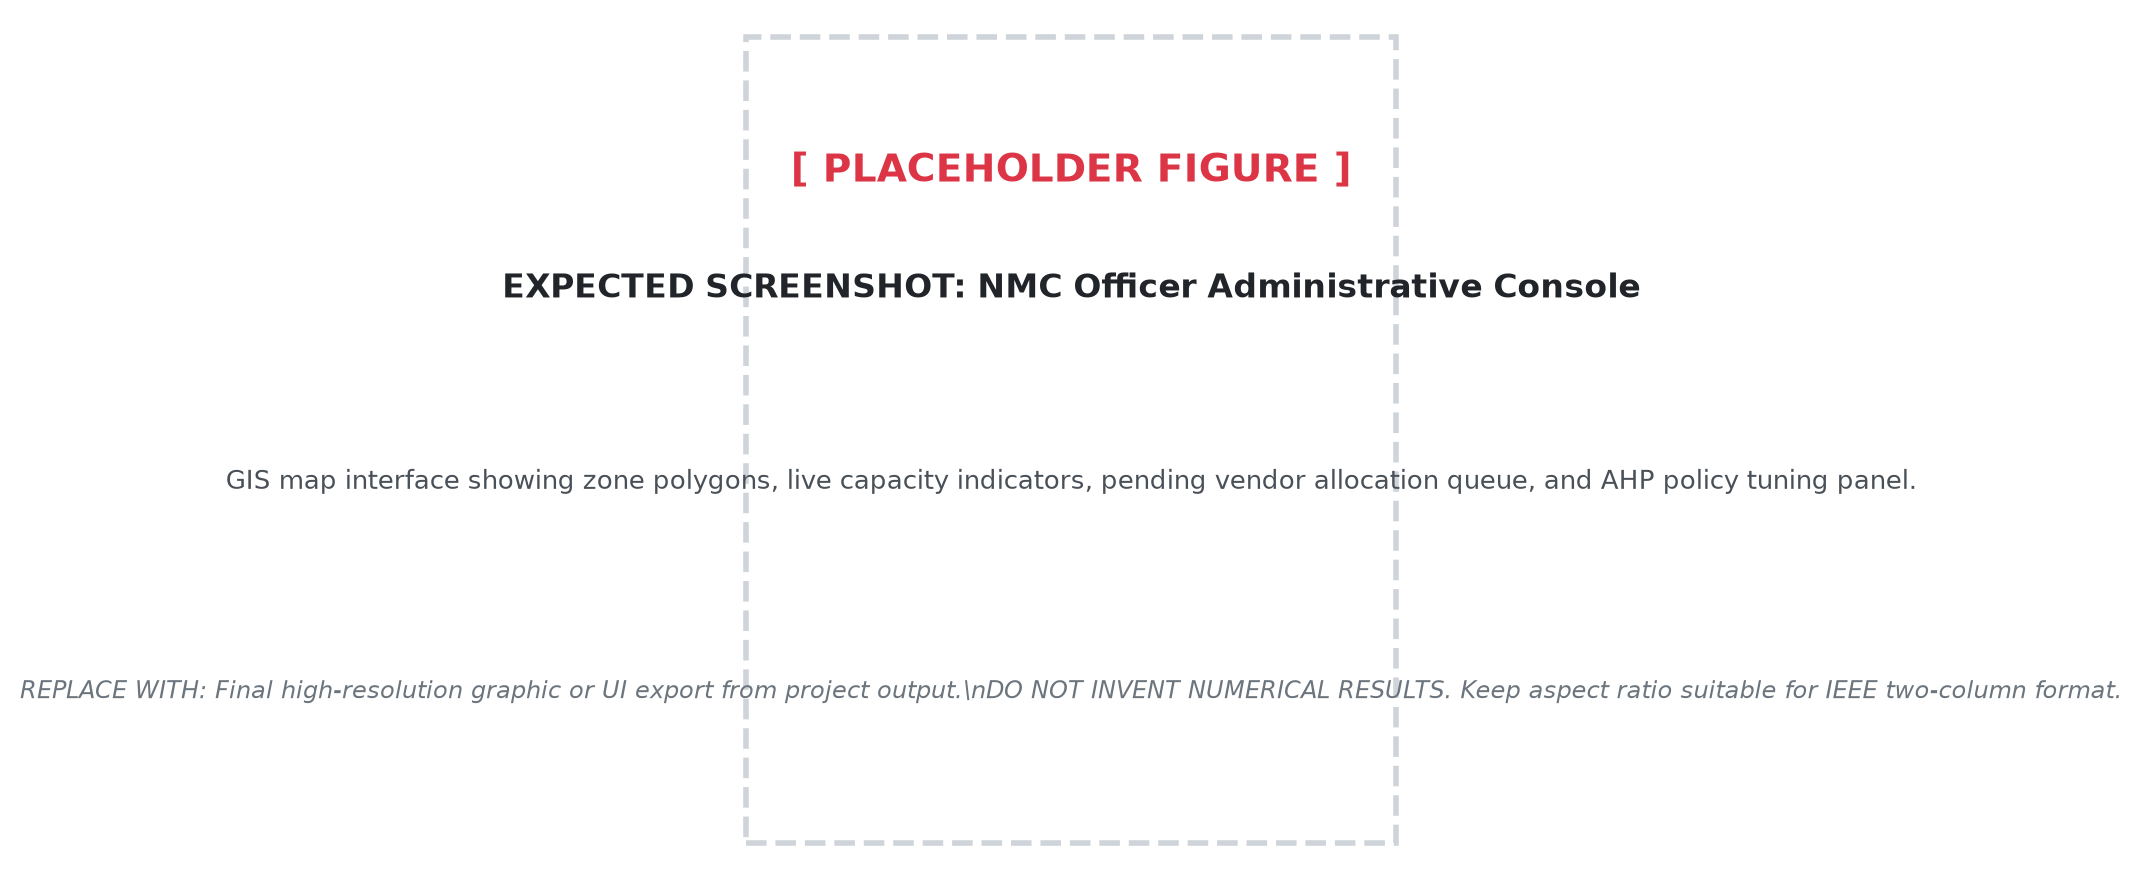
\includegraphics[width=\columnwidth]{figures/placeholders/ui_admin_dashboard_placeholder.png}
    \caption{NMC town-planning officer console showing GIS zone polygons, live capacity indicators, and pending allocation review queues.}
    \label{fig:ui_admin}
\end{figure}

\subsection{Multilingual Vendor Web Portal}
\label{sec:impl_vendor_ui}

To ensure accessibility across linguistic backgrounds, the vendor web portal provides complete internationalization (\texttt{i18n}) supporting both English and Marathi (the regional language of Maharashtra).

\begin{figure}[t]
    \centering
    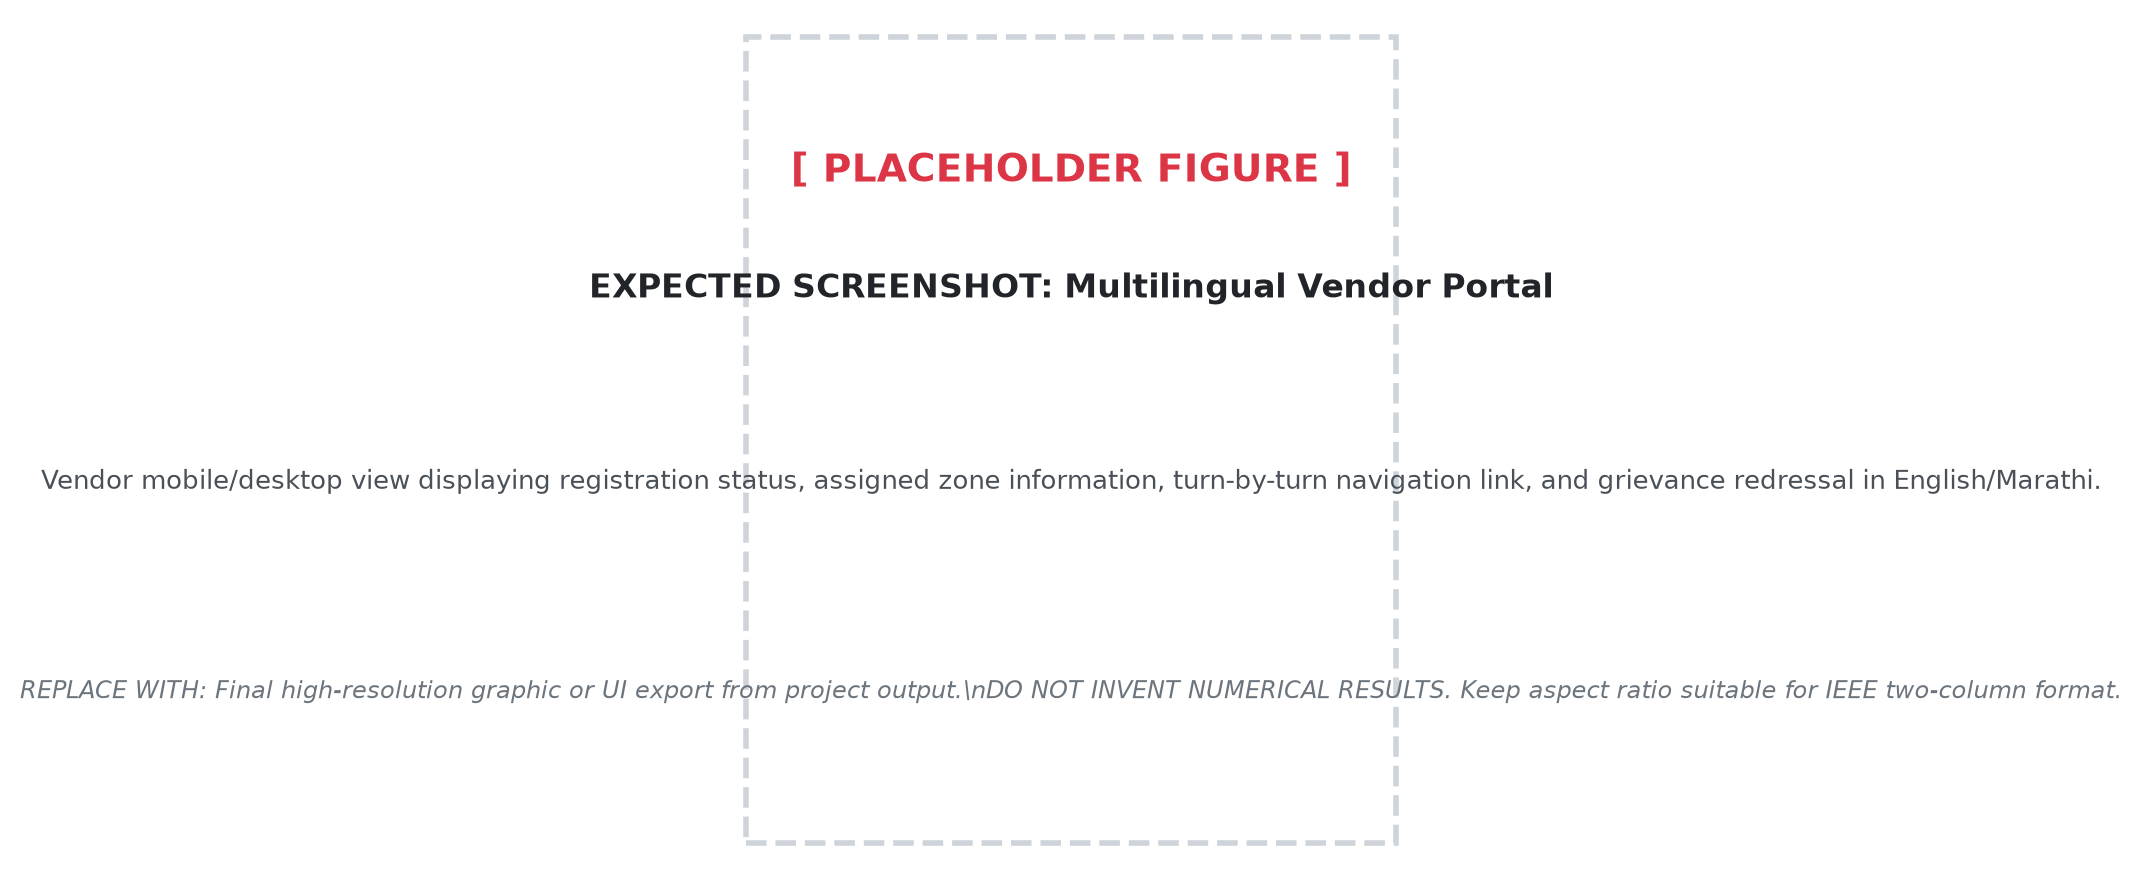
\includegraphics[width=\columnwidth]{figures/placeholders/ui_vendor_portal_placeholder.png}
    \caption{Vendor mobile web portal displaying registration status, assigned zone details, and turn-by-turn navigation guidance in English and Marathi.}
    \label{fig:ui_vendor}
\end{figure}

Key vendor functionalities include:
\begin{itemize}
    \item \textbf{Allocation Status and Digital Credential:} Authenticated vendors can inspect their assigned zone, designated micro-slot identifier (e.g., \texttt{S003}), authorized business category, and permit validity period.
    \item \textbf{Integrated Pedestrian Navigation:} Connects assigned slot coordinates directly to routing engines via Leaflet and GPS geolocators, providing precise turn-by-turn walking directions to the designated $2\,\text{m} \times 2\,\text{m}$ vending footprint.
\end{itemize}

\subsection{Direct Meta WhatsApp Cloud API Conversational Interface}
\label{sec:impl_whatsapp}

Recognizing that many informal vendors face barriers in navigating web browsers or installing mobile applications, UrbanVending AI incorporates an official, direct integration with the Meta WhatsApp Cloud API (Graph API).

\begin{figure}[t]
    \centering
    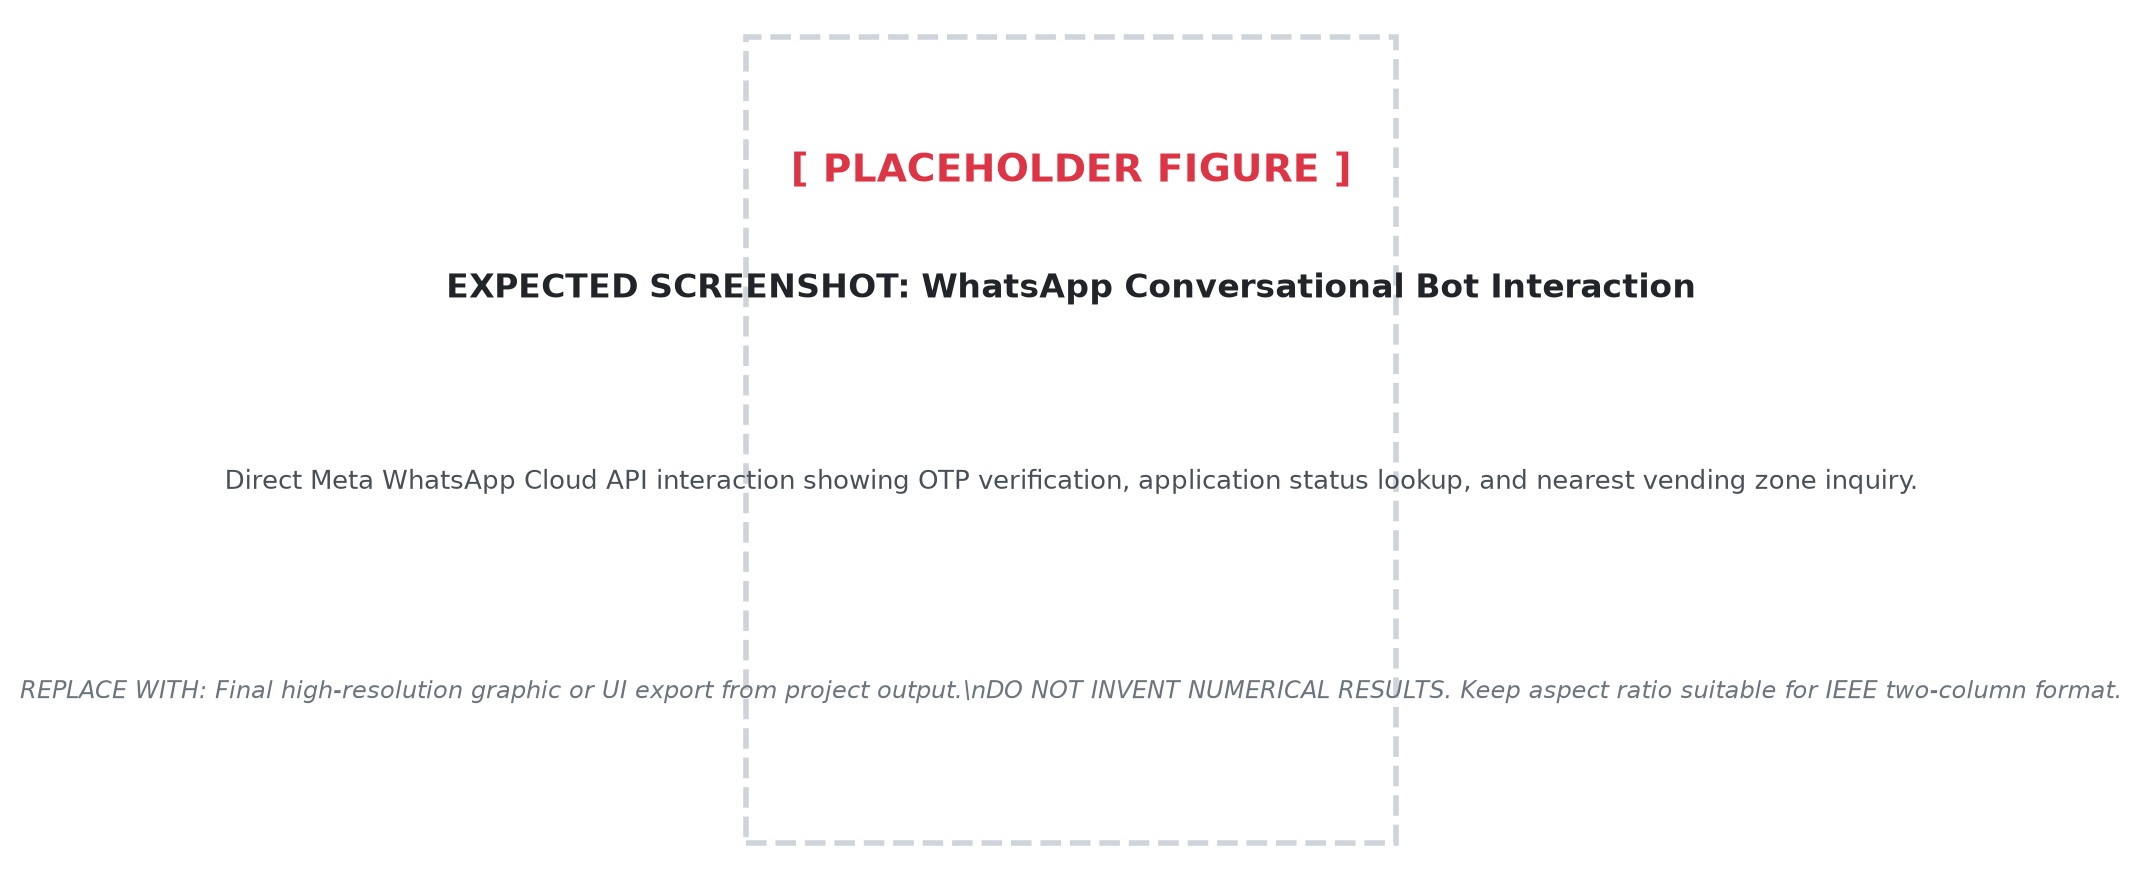
\includegraphics[width=\columnwidth]{figures/placeholders/ui_whatsapp_bot_placeholder.png}
    \caption{Conversational interaction via Meta WhatsApp Cloud API for vendor OTP authentication, status inquiry, and nearby zone discovery.}
    \label{fig:ui_whatsapp}
\end{figure}

The WhatsApp service operates entirely without third-party automation wrappers:
\begin{itemize}
    \item \textbf{Cryptographic Webhook Validation:} Inbound notifications from Meta are verified using HMAC-SHA256 signatures evaluated against \texttt{META\_APP\_SECRET} via the \texttt{X-Hub-Signature-256} header.
    \item \textbf{Persistent Conversational State Machine:} A dedicated conversation state engine in SQLite tracks multi-turn dialogue, enabling vendors to request OTP verification, check application status, locate nearest eligible zones, and register grievances via natural chat interactions.
    \item \textbf{Idempotent Message Deduplication:} Inbound message IDs are deduplicated to prevent double-processing under network retries.
\end{itemize}
